\chapter{Entorno Empresarial}
\thispagestyle{empty} % Quitar el número

En este capítulo se describe el entorno empresarial en el cual tuvo lugar el desarrollo del proyecto de pasantía, la empresa Fischer, Knoblauch \& Co (FKC) filial de Frankfurt.
\section{Fischer, Knoblauch \& Co.}

Es un proveedor de servicios multimedia especializado en el área de aprendizaje electrónico. Está presente en Frankfurt y Munich en Alemania asi como en Basel, Suiza. Fundada en 1996 por Guy Fischer y Thomas Knoblauch.

Proveen consultoria en la integración y ampliación del aprendizaje electrónico a compañias de diversos sectores en Alemania y Bélgica. Se encargan de sugerir la elección de tecnologías, concepción del plan de aprendizaje, didácticas y metódologia de la enseñanza, producción del contenido audiovisual, hasta la integración de la solución en el ambiente del cliente. 

Basicamente, si una compañia requiere enseñar una cierta habilidad a sus empleados contacta a un proveedor de servicios de aprendizaje electrónico, FKC en este caso, los ayuda a integrar un plan aprendizaje a su empresa, que se ven materializados en entrenamientos basados en la web. 

Además FKC haciendo uso de su departamento gráfico y programadores también provee servicios de posicionamiento empresarial en la web, mediante la creación de páginas, logos y demás contenido multimedia que la compañia requiera. 

Sus programadores día a día se enfrentan con diversos retos informáticos en distintos lenguajes de programación. Estos pueden ser: migraciones de sistemas de bases de datos, internazionalización de sus aplicaciones que llegan a estar hasta en 10 lenguajes distintos, diseño de soluciones multiplataforma y el manejo e instalación de Frameworks que faciliten la construcción de soluciones multimedia.

\section{Estructura organizacional}

En la figura \ref{fig:estructuraFKC} se muestra la estructura organizacional de FKC Frankfurt:

\begin{figure}[h]
\begin{center}
	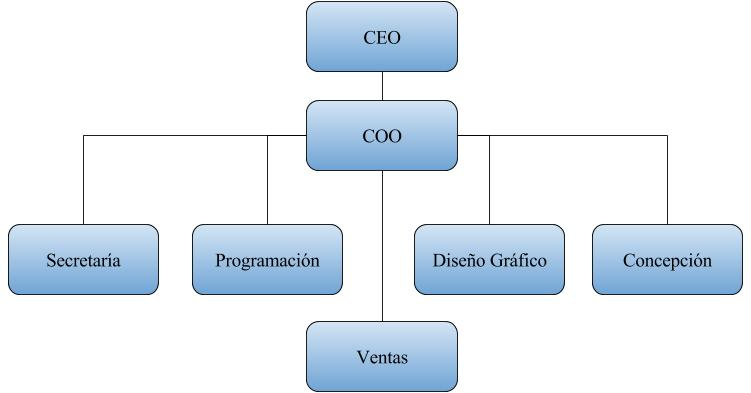
\includegraphics[width=\textwidth]{figuras/estructuraFKC.jpg}
	\caption{Estructura organizacional de FKC.} \label{fig:estructuraFKC}
\end{center}
\end{figure}

FKC Frankfurt es un equipo multidiciplinario donde es importante la comunicación entre los distintos \emph{stakeholders}, los creadores de concepto, se unen a los diseñadores y los programadores para plasmar fielmente los requerimientos del cliente para obtener como resultado una solución hecha a la medida.

\section{Cargo ocupado por el pasante} 

El pasante perteneció al grupo de programación que se muestra en la figura \ref{fig:estructuraFKC} donde formó parte de un equipo de 6 programadores.



